\chapter{Magyarázatgenerálás}\label{ch:exp}
%Diverse feature visualizations reveal invariances in early layers of  deep neural networks
%https://arxiv.org/abs/1807.10589v1
%Feature Visualization
%https://distill.pub/2017/feature-visualization/
%What Uncertainties Do We Need in Bayesian Deep Learning for Computer Vision?
%https://arxiv.org/pdf/1703.04977.pdf

A modern rendszerekben a tesztelésre nagy hangsúlyt fordítanak, főleg ha biztonságkritikus rendszerekről van szó. De a gépi tanulás területe tesztelhetőség szempontjából sajnos jelentősen le van maradva a klasszikus megoldásokkal szemben. Míg egy konvencionális program esetében használhatók egység, modul, integrációs tesztek, formális verifikáció és még sok más, a használt algoritmusok helyessége általában bizonyított és bár kimerítő tesztelés legtöbbször nem lehetséges, gyakran biztosítható hogy a kimenet meghatározott keretek közt marad. Ezzel szemben,például egy neurális háló esetén alap esetben csak a konkrét bemenetekre adott választ tudjuk vizsgálni, ez több szinten is problémás. A tesztre használható példák száma limitált, többet előállítani belőlük költséges, vagy zárt határidőn belül potenciálisan lehetetlen is. A meglévő példáknak is csak egy kis hányadát használhatjuk tesztelésre, mivel szét kell őket osztani tanító,validációs és teszt halmazokra. Mindez azt eredményezi, hogy a bemenetek teljes állapotterének nagyon elenyésző hányadát van kapacitás tesztelni. Ezen kívül zajosak lehetnek a példák, azaz bizonyos tulajdonságok, amik a valóságban sokkal kevésbé, vagy egyáltalán nem korrelálnak a célváltozóval, a véletlen folytán nagy korrelációt mutatnak a rendelkezésre álló adatbázisban. Például képek osztályozásánál az kategorizálandó objektumokat ábrázoló képekben a háttérnek lehet valami sajátossága, esetleg egy bizonyos kategóriába tartozó képek azonos napszakban, azonos éghajlaton, vagy más karakterisztikájú kamerával lettek felvéve, mint a többi példa. Ekkor a hálózat lehet hogy nem a vizsgálandó objektum, hanem annak háttere alapján kategorizálja be a képeket. Többek közt az ilyen zajok felfedezésére használható a magyarázat generálás.

\section{Általánosságban}
%TODO megnézni hogy a bevezetőben ezt hogy írtam.

A magyarázat generálási módszerek két fő kategóriába sorolhatóak, képeket feldolgozó hálózatok esetén alkalmazott a tulajdonság vizualizáció módszere és az általánosan is alkalmazható attribution módszere (magyarul hozzátulajdonítás). 

\subsection{Tulajdonság vizualizáció}

Legfőképpen a mély neurális hálózatoknál alkalmazott, gradiens módszerekre alapuló magyarázat generálási típus. Alap koncepciója hogy már egy célra betanított hálózatra vagy annak egy bizonyos részére meghatároz egy hibafüggvényt, majd a bemenetet úgy módosítja, hogy a kimenet hibája csökkenjen. Tulajdonképpen egy hibavisszaterjesztés algoritmust használva nem a súlyok, hanem a bemeneti értékek parciális deriváltjait határozza meg.

\begin{figure}[H]
    \centering
    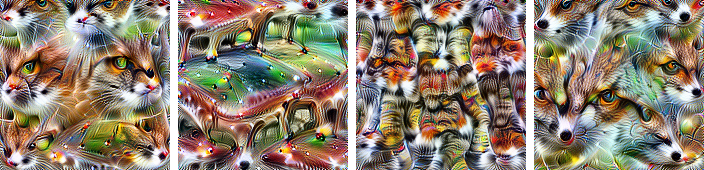
\includegraphics[width=\linewidth]{figures/feature_visualization.png}
    \caption{GoogleNet hálózat 4e inception moduljának egy vizualizációja}
    \label{fig:featurevisualization}
\end{figure}

A hibafüggvény általában arra optimalizál, hogy minél magasabb értéket vegyen fel egy neuron vagy réteg kimenete, ezáltal olyan képet létrehozva amit "érdekesnek talál" a háló.

A kiinduló állapotként gyakran alkalmaznak véletlen bemenetet és példákat is. A példák használatára valid kritika, hogy nem lehet tudni az eredmény milyen mértékben a háló belső karakterisztikája és milyen mértékben csak a bemenet egy torzítása. Másik probléma, hogy egy kép nem reprezentatív a háló működésére, mert nem csak arra a mintára vagyunk kíváncsiak amire leginkább aktiválódik a vizsgált hálózatrész, hanem azokra is amikre kevésbé aktiválódik, de még fontosnak találja őket. Erre a problémára nem kielégítő megoldás több véletlen állapotból indítani az optimalizációt, mivel gyakran nagyon hasonló eredmények alakulnak ki. 

A hiba függvény olyan módú változtatása, hogy penalizálja a korábbiakhoz hasonló képeket javít a képek sokszínűségén, de a képek közti különbség számolásnak is vannak korlátai (például azonos minták jelenléte felcserélve nagy távolságot eredményez), ezért így sem lehet konzisztensen előállítani az összes lényeges mintát.

\subsubsection{Értékelés}

A tulajdonság vizualizáció segít intuíció szerzésében a hálók belső működésével kapcsolatban, ez nagyon értékes, mivel ez segíti a kutatókat is, hiszen megértés nélkül a kutatás csupán vak próbálkozások sorozata. Ezen kívül vizuálisan és érdekesek, ami közelebb hozhatja az embereket a gépi tanuláshoz. Viszont a bevezetőben felvázolt célra nem a legmegfelelőbbek. Ennek oka, hogy maguk az eredmények nehezen értelmezhetőek, ezért ha még tartalmaznak is utalást egy problémára a tanításban, az nehezen lesz megfogható. Továbbá ezek a módszerek nagyrészt specifikusak a háló implementációjára (kivéve ha a kimenetet tekintjük, de annak is megvannak a saját problémái), ezért széles körű alkalmazásuk is nehézkes.

\section{Attribúció (attribution)}

Ezen módszer kimenetekhez bemeneti attribútumokat tulajdonít, ezáltal mutatva, hogy mely bemenetek fontosak a feldolgozásban. Tulajdonképpen megmagyarázza, hogy egy bemenetnél mire alapozta döntését a modell. Erre a célra több alapvetően különböző módszer létezik.

\subsection{Visszaterjesztés alapú attribúció}

Alapvetően ezen módszerek a háló hibafüggvényének a bemenetek szerint vett gradiensét veszi alapul. Azonban a tulajdonság vizualizációs módszerekkel ellentétben nem változtatja a bemeneti értéket a gradiens alapján. 

% http://proceedings.mlr.press/v70/sundararajan17a.html
Egy ilyen módszer az integrált gradiens módszere, mely minden bemeneti értéket egyenként a példában adott érték és 0 (vagy más megadott érték) közt vett lineáris skála alapján variálja, és az így kapott átlagos derivált érték lesz a tulajdonság fontossági értéke. Ezen algoritmus egy felhasználási módja látható \aref{fig:grading} ábrán.

%kép
%http://proceedings.mlr.press/v70/sundararajan17a.html
\begin{figure}[H]
    \centering
    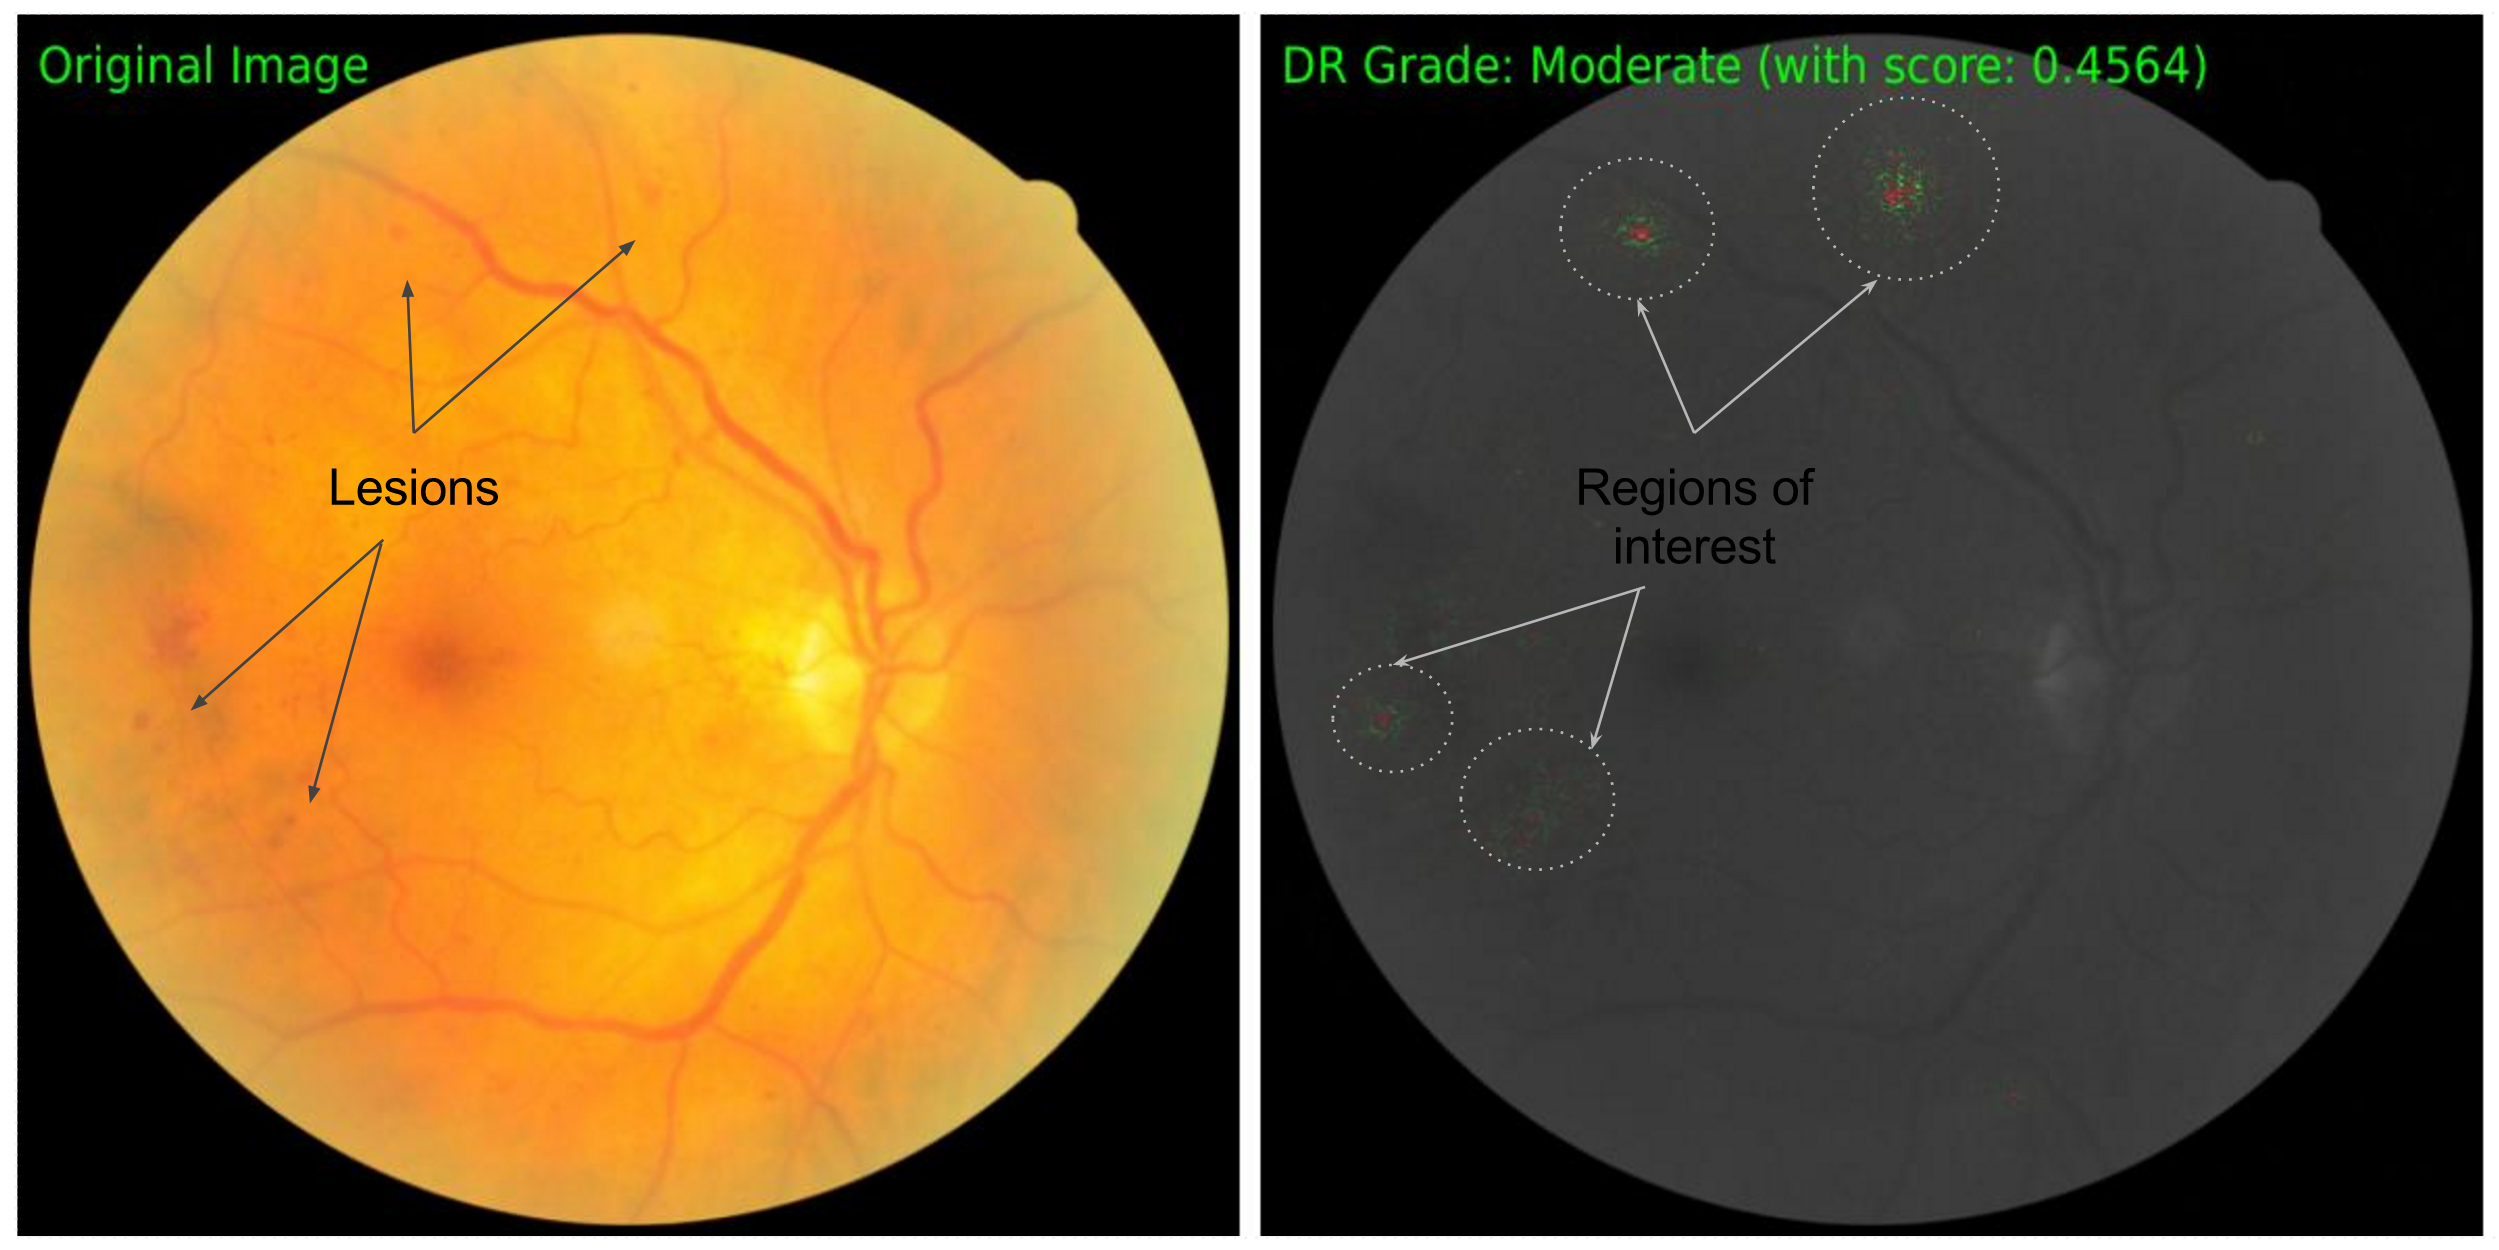
\includegraphics[width = \textwidth]{figures/grading.png}
    \caption{Diabetikus betegek retináján sérüléseket kereső hálózat integrált gradiens alapú magyarázata}
    \label{fig:grading}
\end{figure}

%TODO n és N helyet l és L el indexelni a rétegeket mindenhol

Egy másik algoritmus a deepLIFT (Deep Learning Important FeaTures) amely egy rétegenkénti fontosság propagáló algoritmus. A lényege, hogy a kimenettől visszafelé egy frissítési szabály alapján határozza meg az $r^{(n)}_i$ fontosság értéket. Először forward passt végez egy referencia értékkel (általában null-vektor) és elmenti a forward pass részeredményeit, ahol a rétegek referencia kimenete $\bar{y}^{(n)}$.

\begin{subequations}
    \begin{equation}
         r^{(n)}_i = \sum_j \cfrac{z_{ji}^{(n)}-\bar{z}_{ji}^{(n)}}{\sum_{i'} z_{ji}^{(n)} - \sum_{i'} \bar{z}_{ji}^{(n)}} r^{(n+1)}_j
         \label{deepLIFT}
    \end{equation}
    \begin{equation}
        \text{, ahol } z^{(n)}_{ji} = w_{ji}^{n+1} y_i^{(n)} \text{ és } \bar{z}_{ji}^{(n)} = w_{ji}^{n+1} \bar{y}_i^{(n)}
    \end{equation}
    
\end{subequations}
Az egyenlet lényegében összegzi, hogy a következő réteg neuronjai mennyire tartják fontosnak a vizsgált neuron bemenetét, szorozva azzal hogy ők maguk mennyire fontosak. 

Itt ${z}_{ji}^{(n)}$ tekinthető két neuron közti kapcsolat erejének, ami nem csak attól függ hogy mekkora súly tartozik a bemenethez, hanem attól is hogy a vizsgált példa esetén érkezik-e "információ" a kapcsolaton keresztül, azaz a bemenet mennyire tér el a nullától. A bias értékek miatt nullvektor bemenetkor nem feltétlenül nullák a a fontosságok, ami torzíthat az eredményen. $\bar{z}_{ji}^{(n)}$ érték itt ezt a torzítást hivatott kiküszöbölni, segítségével \aref{deepLIFT} egyenlet nulla fontossági értéket rendel a referenciával megegyező fontosság esetén. Ez az érték még el van osztva egy arányosító faktorral, ami azt adja meg hogy a következő réteg $j$ indexű neuronja összességében mennyire tartja fontosnak bemeneteit, hiszen egy neuron aminek minden súlya 10000 nem szabad hogy aránytalanul nagy súllyal szerepeljen a többi neuron szerinti fontossághoz képest.

Ezt az összefüggést rétegenként visszafelé alkalmazva a hálózaton, megkapjuk minden neuron fontossági értékét, de a lényeges végeredmény az a bemeneti réteg neuronjainak, azaz a bemeneti tulajdonságoknak a fontossága. 

\subsubsection{Értékelés}
A gradiens módszerek elméleti szinten korlátozva vannak hibavisszaterjesztést alkalmazó gépi tanulási módszerekre, implementációs korlátok miatt pedig gyakran konkrét rendszerekre külön kell őket illeszteni. Ez felhasználhatósági kör szempontjából erősen korlátozó tényező. Viszont van olyan attribúciós módszer ami ezzel a problémával nem küzd.

\subsection{Perturbáció alapú attribúció}

A magyarázat generálási módszerek ezen kategóriája black boxként is képes kezelni a hálózatokat. A módszer alapja, hogy egy konkrét példának a tulajdonságait megváltoztatja és fontosságát a kimenetben történt változás alapján határozza meg. Első hallásra a gradiens számolás átfogalmazásának  hangozhat és bár bizonyos esetekben közelítheti azt, több lehetőséget kínál. Egyszerre akár több tulajdonság is változhat, így vizsgálhatjuk a tulajdonságok egymásra hatását. Ha nagyon kis mértékben változtatunk egy tulajdonságon akkor valóban közelítjük a deriváltját, de például kategorikus tulajdonságoknál elképzelhető hogy pontatlan fontossági értéket jelent a derivált, hiszen csak diszkrét bemenetek értelmezettek.

A tulajdonságok módosítása több módon is történhet. Kategorikus esetben néhány vagy az összes érték tesztelésével, folytonos értékeknél meghatározott értelmezési tartományban mintavételezés alapján. Ez a tartomány gyakran a tanító példákból meghatározott legtágabb értelmezési tartomány. Számítási kapacitás szempontjából előnyös lehet a maszkolás módszere. Ekkor csak két értéket vehet fel egy tulajdonság, a példában találhatót és egy referencia értéket. Ez a referencia gyakran nulla, vagy képek esetén a szürke színnek megfelelő intenzitás.

Léteznek megoldások amik más információkat is kihasználnak, de ezen módszerek csupán a bemenet és kimenet vizsgálatával is képesek magyarázatok előállítására. Ez lehetővé teszi olyan eszközök létrehozását melyek bármilyen gépi tanulási modell magyarázatára képesek, legyen az neurális hálózat, SVM, döntési fa alapú megoldások és sok más. Ez a tulajdonság a modell-agnosztikusság. 

Arra, hogy a perturbációból kapott eredményekből milyen módon jön létre a magyarázat több megoldás létezik. Egyszerűen tekinthetjük fontosságnak, hogy milyen mértékben változott a kimenet a perturbálás hatására, ahogy azt több korábban bemutatott algoritmus is tette. Komplexebb megoldás ha a perturbáció után keletkezett bemenet-kimenet párokat tanító adathalmazként tekintjük és a feladatra alkalmas gépi tanulási modellt tanítunk vele. Ez a modell a magyarázandó modell működését lokálisan közelíti, ahol a lokalitás mértéke a perturbációtól függ. Ez a modell viszont csak akkor alkalmas a feladatra, ha önmagában magyarázatként használható. Ezt, és több más attribúciós módszert is felhasználó keretrendszer a LIME, amit \aref{ch:lime} fejezet részletez.